\lecture{16}{Free Energy}{Qiang Zhu}{scribe-name1,2,3}

\section{Free Energy as a Force toward Equilibrium}
For an isolated system, the entropy tends to increase. The system's entropy determines the direction of spontaneous change. 
But what if a system is not isolated? Now energy can pass between the system and the environment. The 2nd law still applies.
However, the total entropy would be the determining factor.

Let's consider a small change in the total entropy;
\begin{equation} dS_\text{total} = dS + dS_R \end{equation}

Applying the thermodynamic identity, we get,
\begin{equation} dS = \frac{1}{T}dU + \frac{P}{T}dV - \frac{\mu}{T}dN \end{equation}

if we assume $N$ and $V$ is fixed, we have
\begin{equation} dS_\text{total} = dS + \frac{1}{T}dU_R \end{equation}
Since $T$ is in equilibrium,
\begin{equation} dS_\text{total} = dS - \frac{1}{T}dU \end{equation}
Therefore,
\begin{equation} dS_\text{total} = -\frac{1}{T}(dU-TdS) = -\frac{1}{T}dF \end{equation}
Finally, we come to the conclusion that the increase of $S$ is equivalent to the decrease in $F$, under constant $N, V, T$ conditions.
This allows us to forget about the reservoir and just consider the free energy itself.
Similarly, we can derive the relation under constant $N, P, T$ conditions,
\begin{equation} dS_\text{total} = -\frac{1}{T}(dU-TdS+PdV) = -\frac{1}{T}dG \end{equation}

Let me summarize these points,
\begin{enumerate}
\item constant $V, T$ $\rightarrow$ $S$ tends to increase
\item constant $N, V, T$, $\rightarrow$ $F$ tends to decrease
\item constant $N, P, T$, $\rightarrow$ $G$ tends to decrease
\end{enumerate}

Reconsider the case of burning water:~~~~~~~\ce{H2 + 1/2 O2 -> H2O}\\

\section{Various Phase Transitions}
Phases: Different forms of the substance, such as liquid, gas, solid.\\
A phase transformation is a discontinuous change in the properties of a substance.\\
1st order $\rightarrow$ the discontinuous changes of properties is the 1st derivative of energy\\
2nd order $\rightarrow$ the discontinuous changes of properties is the 2nd derivative of energy\\
Some key points in the phase diagram,
\begin{enumerate}
\item phase boundary, 
\item triple point, where solid, liquid, gas coexists
\item slope of phase boundary, ice anomaly
\item critical points, where gas and liquid are no longer distinguishable (fluid)
\item superconducting......
\item Curie temperature
\end{enumerate}

Diamond/Graphite
\begin{equation} 
(\frac{\partial G}{\partial P})_{T,N} = V
\end{equation}

\begin{equation} 
(\frac{\partial G}{\partial T})_{P,N} = -S
\end{equation}



\section{The Clausius-Clapeyron Relation}
At the phase boundary, the material is equally stable as a liquid or a gas, so its Gibbs free energy must be the same,
\begin{equation} G_l = G_g \end{equation}
Now imagine increasing the temperature by $dT$ and the pressure by $dP$, in such a way that the two phases remain equally stable.
Under this change,
\begin{equation} dG_l = dG_g \end{equation}
Therefore, by the thermodynamic identify for $G$,
\begin{equation} -S_ldT + V_ldP = -S_gdT + V_gdP \end{equation}
Where $\mu dN$ term is intentionally neglected ($N$ is fixed). 
Now it is easy to solve for the slope of the phase boundary line,
\begin{equation} \frac{dP}{dT} = \frac{S_g-S_l}{V_g-V_l} \end{equation}
Therefore, the slope is determined by the entropies and volumes of the two phases.
Shallow/stiff.
In practice, it is more convenient to write as
\begin{equation} \frac{dP}{dT} = \frac{L}{T\Delta{V}} \end{equation}
where, $L$ is the latent heat for converting the material from liquid to gas. And this is known as the {\bf Clausius-Clapeyron relation}

The $P$-$T$ slope of the solid-liquid phase boundary is usually positive. But water is an exception. Why?\\
Diamond/Graphite, (300 K, 15 kbar) .v.s (1800 K, 60 kbar)\\

Below 0.3 K the slope of the $^3$He solid-liquid phase boundary is negative, which phase is more dense? Which phase has more entropy?\\
Solid phase is denser, and has more entropy.\\
At absolute 0 K, the slope goes to 0, as $\Delta{S}$ goes to 0.\\
From Liquid to Solid, $S$ has to increase.\\
During adiabatic compression, $S$ has to remain constant.\\
Therefore, $T$ has to drop. A good way to reach ultra-low temperature.

\section{Homework}
Problems 5.12, 5.13, 5.14, 5.21, 5.23\\
Problems 5.24, 5.28, 5.29, 5.32, 5.40\\
%{\bf Problem 5.45}, when a rising air mass becomes saturated, the condensing water droplets will give up energy, thus slowing the adiabatic cooling process. Use the first law to show that, as condensation forms during adiabatic expansion, the temperature of an air mass changes by
%\begin{equation}
%dT = \frac{2}{7}(\frac{T}{P}dP - \frac{L}{nR}dn_w,
%\end{equation}
%where $n_w$ is the number of moles of water vapor present, $L$ is the latent heat of vaporization per mol, and $\gamma$ is 7/5 for air. You may assume that the H$_2$O makes up only a small fraction of the air mass.
%
\newpage
\begin{figure}[h]
\centering
\includegraphics[width=12cm]{imgs/water_phase_diagram_2}
\caption{The Phase diagram for H$_2$O. }
\end{figure}

\begin{figure}[ht]
\centering
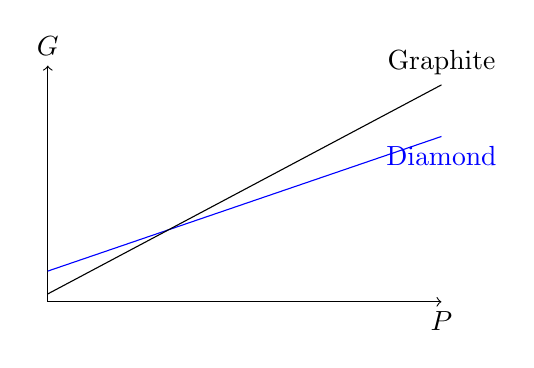
\begin{tikzpicture}%[x=1cm, y=3cm]
\draw [->] (0,0) -- (0, 3) node[above]{$G$};
\draw [->] (0,0) -- (5, 0)  node[below]{$P$};
\draw [color=blue, domain=0:5]  plot(\x, {0.39 + 0.342*\x}) node[below] {Diamond};
\draw [color=black,domain=0:5]  plot(\x, {0.10 + 0.531*\x}) node[above] {Graphite};
\end{tikzpicture}
\caption{Graphite versus diamond.}
\end{figure}


